% Provenance (never printed): see sources/outline_sources.md (Year 2: interstellar
% medium, molecular clouds, gravitational collapse and the Jeans criterion, protostars
% and protostellar discs). Curves from figdata/bachelor-2/jeans.py; exercise and problem
% values in the Book 4 scratch calculator calc/ch01.py.
\chapter{Le milieu interstellaire et la formation des étoiles}\label{ch:b2:ism-star-formation}

Dans la constellation du Taureau, à environ \qty{140}{\parsec} du Soleil, une tache sombre
masque les étoiles situées derrière elle. Observée avec un radiotélescope réglé sur les raies du monoxyde de carbone, la tache est un nuage de gaz froid environ vingt mille fois plus
massif que le Soleil, parsemé de filaments~; au cœur de ses grumeaux les plus denses naissent de jeunes étoiles, et autour de l'une d'elles, HL Tauri, un disque de poussière présente une alternance d'anneaux clairs et sombres où des planètes se forment peut-être déjà.
Le Soleil, la Terre et chaque atome des roches de ce livre ont un jour été contenus dans un tel nuage. Ce chapitre suit la matière d'un système planétaire depuis le gaz ténu qui s'étend entre les étoiles jusqu'à un disque autour d'une étoile nouvellement née~: ce qu'est le \omterm{def:b2:ism-star-formation:ism}{milieu interstellaire}, pourquoi un nuage soutenu par sa propre chaleur finit par s'effondrer,
combien de temps dure cet effondrement, comment une étoile rassemble sa masse et pourquoi la matière qui ne tombe
pas
sur
elle
finit
dans
un
disque.

\begin{recall}
Une étoile de la séquence principale brille en fusionnant l'hydrogène en hélium dans son cœur
et se maintient par sa pression contre son propre poids~; sa position dans le diagramme de Hertzsprung--Russell est fixée par sa masse (les volumes de physique, troisième année
universitaire). Un corps en orbite fermée autour d'une masse $M$ obéit à la troisième loi de Kepler, $T^2 = 4\pi^2 a^3/(GM)$ (les volumes de physique, première année universitaire). Un corps noir de température $T$ émet $\sigma T^4$ par unité de surface (les volumes de
physique, deuxième année universitaire). Dans un gaz parfait de $N$ particules, l'énergie cinétique moyenne de translation vaut $\tfrac32 N k_{\mathrm B} T$. Le parsec, \qty{3.086e16}{m}, est l'unité de distance du
volume
de
première
année
universitaire.
\end{recall}

\section{La matière entre les étoiles}

L'espace entre les étoiles n'est pas vide. Près du Soleil, il contient en moyenne environ
un atome d'hydrogène par centimètre cube, soit une densité de masse de \qty{2.7e-24}{g.cm^{-3}}~; l'air que nous respirons contient environ $10^{19}$ fois
plus de molécules dans le même volume (\cref{exo:b2:ism-star-formation:1}). Répandue dans la Galaxie, cette matière ténue représente encore \qtyrange{10}{15}{\percent} de la masse
du
disque
galactique.
% ledger: ferriere:mean-density, ferriere:disc-fraction

\begin{definition}[Milieu interstellaire, poussière interstellaire]
\label{def:b2:ism-star-formation:ism}
Le \emph{milieu interstellaire}\index{milieu interstellaire} est le gaz et la poussière qui
remplissent l'espace entre les étoiles d'une galaxie. La \emph{poussière interstellaire}\index{poussière interstellaire} en est la part sous forme de grains solides, de quelques
nanomètres à environ un micromètre de diamètre, faits de silicates, de composés carbonés et, dans les régions froides,
de
glaces.
\end{definition}

Sa composition est celle que l'on mesure dans le Soleil et dans les météorites~: en
masse, \qty{70.4}{\percent} d'hydrogène, \qty{28.1}{\percent} d'hélium et \qty{1.5}{\percent} d'éléments plus lourds. Seuls \qtyrange{0.5}{1}{\percent} de la
masse sont dans la poussière, mais celle-ci détient l'essentiel de certains éléments~: le gaz est plus pauvre que le Soleil en magnésium, en silicium et en fer, d'un facteur 10 à 100, parce que ces atomes sont enfermés dans les grains, tandis que
le carbone, l'azote et l'oxygène ne sont appauvris que d'un facteur 1.2 à 3. Les grains sont les premiers solides d'un futur
système
planétaire~;
\cref{ch:b2:planet-formation-meteorites}
les
suit.
% ledger: ferriere:composition, ferriere:dust-fraction, ferriere:refractory-depletion

\subsection{Cinq phases}

Le gaz est loin d'être uniforme. Il se présente en quelques états distincts, ou phases,
chacun avec son propre domaine de température et de densité (tableau ci-dessous). Environ la moitié de sa masse est dans des nuages qui n'occupent que \qtyrange{1}{2}{\percent}
du volume~; le reste, tiède ou chaud, remplit l'espace entre
eux.
% ledger: ferriere:disc-fraction

\begin{table}[htbp]
\centering
\small
\begin{tabular}{lll}
\hline
phase & température (K) & densité $n$ (\unit{cm^{-3}}) \\
\hline
moléculaire & 10--20 & $10^2$--$10^6$ \\
atomique froid & 50--100 & 20--50 \\
atomique tiède & 6000--10\,000 & 0.2--0.5 \\
ionisé tiède & environ 8000 & 0.2--0.5 \\
ionisé chaud & environ $10^6$ & environ 0.0065 \\
\hline
\end{tabular}
\caption{Les phases du gaz interstellaire près du Soleil~; $n$ est la densité
de noyaux d'hydrogène.}
\label{tab:b2:ism-star-formation:phases}
% ledger: ferriere:molecular, ferriere:cold-atomic, ferriere:warm-atomic, ferriere:warm-ionized, ferriere:hot-ionized
\end{table}

Le tableau cache une régularité. La pression d'un gaz parfait vaut
$P = n k_{\mathrm B} T$, de sorte que le produit $nT$ la mesure. Pour le gaz atomique froid, $nT$ vaut environ $30\times75 \approx 2000$ (en \unit{K.cm^{-3}}),
pour le gaz atomique tiède environ $0.3\times8000 \approx 2400$, pour le gaz chaud environ $0.0065\times10^6 = 6500$~: à un facteur de quelques unités près, les trois phases qui se partagent l'espace entre les nuages sont à la même pression (figure
ci-dessous). Là où un gaz chaud et un gaz froid se touchent à pression égale, aucun ne repousse l'autre~; un gaz qui se refroidit à pression constante devient plus dense en proportion et passe de la phase tiède à la phase froide. Les \omterm{def:b2:ism-star-formation:molecular-cloud}{nuages moléculaires} atteignent des pressions bien plus élevées, jusqu'à des milliers de
fois plus dans leurs parties denses~: ils sont liés par leur propre gravité, et non par
la
pression
de
leur
environnement.

\begin{omfigure}
\begin{tikzpicture}
\begin{axis}[omrecord, width=0.86\linewidth, height=6.4cm, xmode=log, ymode=log,
  xmin=1e-3, xmax=1e7, ymin=3, ymax=3e6,
  xlabel={densité de noyaux d'hydrogène $n$ (\unit{cm^{-3}})}, ylabel={température $T$ (K)},
  tick label style={font=\scriptsize}, label style={font=\small}, clip=false,
  legend pos=north east, legend style={font=\scriptsize, draw=black!30}]
\addplot[black!45, densely dashed, domain=1e-3:1e3, samples=2] {3000/x};
\addlegendentry{$nT = \num{3000}$}
\addplot[black!60, densely dotted, thick, domain=0.1:1e5, samples=2] {3e5/x};
\addlegendentry{$nT = 3\times10^5$}
\fill[blue!45, opacity=0.6] (axis cs:1e2,10) rectangle (axis cs:1e6,20);
\fill[teal!50, opacity=0.6] (axis cs:20,50) rectangle (axis cs:50,100);
\fill[orange!55, opacity=0.6] (axis cs:0.2,6000) rectangle (axis cs:0.5,10000);
\fill[red!45, opacity=0.6] (axis cs:0.2,5714) rectangle (axis cs:0.5,11200);
\fill[violet!50, opacity=0.6] (axis cs:0.00464,7.14e5) rectangle (axis cs:0.0091,1.4e6);
\node[font=\scriptsize, anchor=south east] at (axis cs:1e6,20) {nuages moléculaires};
\node[font=\scriptsize, anchor=south west] at (axis cs:50,100) {atomique froid};
\node[font=\scriptsize, anchor=east, align=right] at (axis cs:0.17,8000) {atomique tiède\\et ionisé tiède};
\node[font=\scriptsize, anchor=west] at (axis cs:0.011,1e6) {ionisé chaud};
\end{axis}
\end{tikzpicture}

\par\smallskip{\small Les phases du gaz interstellaire près du Soleil (intervalles du tableau ci-dessus~; les phases
tiède ionisée et chaude, données par une seule valeur, sont tracées sous forme de boîtes d'un facteur 1.4 en largeur). Le long de chaque ligne grise, la pression $nk_{\mathrm B}T$ est constante~: les phases froide,
tiède et chaude se trouvent à peu près à la même pression, à un facteur de quelques unités près,
tandis que les \omterm{def:b2:ism-star-formation:molecular-cloud}{nuages moléculaires}, liés par leur propre gravité, atteignent des pressions jusqu'à des milliers de fois plus élevées.
Données~:
Ferrière (2001).}
\end{omfigure}

La poussière se manifeste de trois façons. Elle assombrit la lumière des étoiles situées
derrière elle, et davantage le bleu que le rouge, si bien que les étoiles vues à travers elle paraissent plus rouges qu'elles ne le sont. Elle rayonne dans l'infrarouge lointain et
aux longueurs d'onde millimétriques, à la température de quelques dizaines de kelvins à laquelle la lumière des étoiles la porte. Et elle cache à l'optique ce qui se trouve à l'intérieur d'un nuage dense~: c'est pourquoi la formation stellaire s'observe dans le domaine
radio et infrarouge. Le gaz se repère par ses raies~: l'hydrogène atomique par sa raie radio à \qty{21}{cm}, l'hydrogène moléculaire, qui rayonne à peine lorsqu'il est froid, par les raies des molécules qui l'accompagnent, le
monoxyde
de
carbone
en
tête.

\section{Nuages moléculaires}

La phase la plus froide et la plus dense est celle où naissent les étoiles.

\begin{definition}[Nuage moléculaire, cœur dense]
\label{def:b2:ism-star-formation:molecular-cloud}
Un \emph{nuage moléculaire}\index{nuage moléculaire} est une région du \omterm{def:b2:ism-star-formation:ism}{milieu
interstellaire} assez dense et opaque pour que son hydrogène soit surtout sous forme de molécules, \ce{H2}, protégées par la poussière de la lumière ultraviolette des
étoiles qui les détruiraient~; sa température est d'environ \qty{10}{K} à \qty{20}{K}. Un \emph{cœur dense}\index{cœur dense} est une condensation compacte à l'intérieur d'un nuage moléculaire, de quelques dixièmes de parsec de diamètre au plus, avec des
densités de $10^4$ à $10^5$ particules par centimètre cube, à partir de laquelle se forme une seule étoile ou
un
petit
groupe
d'étoiles.
\end{definition}

Les nuages s'organisent en hiérarchie (tableau ci-dessous). Un nuage sombre comme celui du
Taureau contient des grumeaux, et les grumeaux contiennent des cœurs, chaque niveau étant plus dense, plus petit et plus calme que le précédent~: dans un cœur, le gaz se déplace au plus
à quelques dixièmes de kilomètre par seconde, la vitesse du son dans un gaz à \qty{10}{K}. La région du Taureau cartographiée dans le monoxyde de carbone contient environ \num{2.4e4} masses solaires de gaz~; seules \qtyrange{0.3}{1.2}{\percent} de celles-ci se sont transformées
en jeunes étoiles observées là-bas, à raison d'environ huit étoiles par cent mille ans au cours des trois derniers millions d'années. La formation stellaire
est
lente
et
gaspilleuse.
% ledger: bt07:clouds, bt07:clumps, bt07:cores, goldsmith:taurus-mass, goldsmith:taurus-sfe, goldsmith:taurus-distance

\begin{table}[htbp]
\centering
\small
\begin{tabular}{lccc}
\hline
 & nuages sombres & grumeaux & \omterm{def:b2:ism-star-formation:molecular-cloud}{cœurs denses} \\
\hline
masse (masses solaires) & $10^3$--$10^4$ & 50--500 & 0.5--5 \\
taille (pc) & 2--15 & 0.3--3 & 0.03--0.2 \\
densité moyenne (\unit{cm^{-3}}) & 50--500 & $10^3$--$10^4$ & $10^4$--$10^5$ \\
température du gaz (K) & environ 10 & 10--20 & 8--12 \\
exemples & Taureau, Musca & --- & L1544, B68 \\
\hline
\end{tabular}
\caption{La hiérarchie d'un \omterm{def:b2:ism-star-formation:molecular-cloud}{nuage moléculaire} sombre. Les densités comptent toutes
les particules. Données~: Bergin et Tafalla (2007).}
\label{tab:b2:ism-star-formation:hierarchy}
% ledger: bt07:clouds, bt07:clumps, bt07:cores
\end{table}

Pourquoi les nuages sont-ils si froids~? Le gaz perd de l'énergie en émettant des
photons qui s'échappent, et les molécules sont d'excellents émetteurs~: une collision porte une molécule de monoxyde de carbone à un niveau de rotation plus élevé, la molécule
redescend en émettant un photon à la longueur d'onde millimétrique, et le photon quitte le nuage en emportant l'énergie de la collision. La poussière, réchauffée par la faible lumière stellaire qui pénètre, rayonne dans l'infrarouge lointain. Le chauffage, dû aux
rayons cosmiques et à la lumière stellaire filtrée par la poussière, est faible~; l'équilibre s'établit près de \qty{10}{K}. Dans un tel gaz la pression thermique est faible,
et
la
gravité
peut
l'emporter.

\begin{omfigure}
\begin{minipage}[c]{0.44\linewidth}
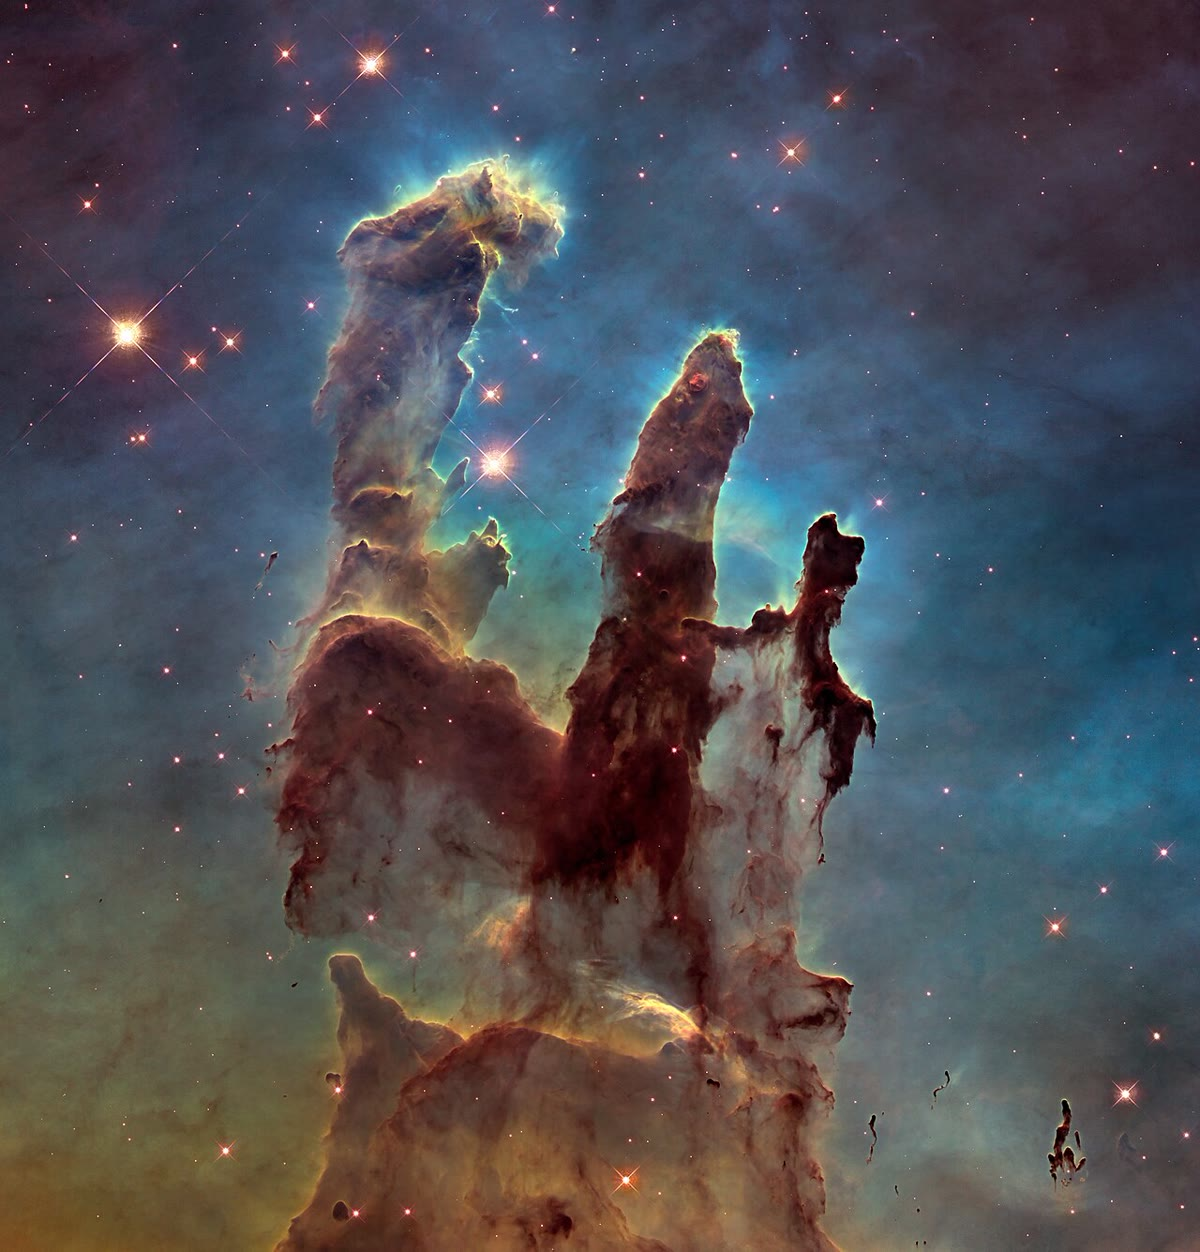
\includegraphics[width=\linewidth]{images/book4/b2-pillars-of-creation.jpg}
\end{minipage}\hfill
\begin{minipage}[c]{0.52\linewidth}
{\small Les « Piliers de la Création » de la nébuleuse de l'Aigle, photographiés par le télescope
spatial Hubble en lumière visible. Les colonnes sont faites de gaz moléculaire froid et dense et de poussière, longues de plusieurs années-lumière, érodées et éclairées par le dessus par la
lumière ultraviolette de jeunes étoiles massives situées hors du cadre~; la poussière les rend opaques. De petites condensations à leurs sommets forment des étoiles. NASA, ESA et Hubble Heritage Team
(STScI/AURA),
domaine
public.}
\end{minipage}
\end{omfigure}

\section{Effondrement gravitationnel}

Un nuage est un équilibre entre deux énergies~: l'énergie thermique de son gaz, qui pousse
vers l'extérieur, et son énergie gravitationnelle, qui tire vers l'intérieur. La seconde croît plus vite avec la masse que la première~; au-delà d'une certaine masse, la
gravité
l'emporte.

\begin{proposition}[Énergie gravitationnelle d'une sphère uniforme]
\label{prop:b2:ism-star-formation:grav-energy}
Une sphère de densité uniforme, de masse $M$ et de rayon $R$, possède
l'énergie potentielle gravitationnelle
\[
  U = -\frac{3}{5}\,\frac{G M^2}{R}.
\]
\end{proposition}

\begin{proof}
Construisons la sphère coquille par coquille. Lorsque son rayon vaut $r$, elle a la
masse $m(r) = M r^3/R^3$~; amener une coquille d'épaisseur $\mathrm dr$, de masse $\mathrm dm = 3M r^2\,\mathrm dr/R^3$, de l'infini à sa surface libère l'énergie
$G m(r)\,\mathrm dm/r$, car une sphère attire à l'extérieur comme si sa masse était concentrée en son centre (théorème des coquilles sphériques, les volumes de
physique).
D'où
\[
  U = -\int_0^R \frac{G}{r}\,\frac{M r^3}{R^3}\,\frac{3 M r^2}{R^3}\,\mathrm dr
    = -\frac{3 G M^2}{R^6}\int_0^R r^4\,\mathrm dr = -\frac{3}{5}\,\frac{G M^2}{R}.
  \qedhere
\]
\end{proof}

Un corps autogravitant en équilibre obéit au théorème du viriel~: en moyenne dans le
temps, deux fois son énergie cinétique plus son énergie gravitationnelle est nulle, $2K + U = 0$ (les volumes de physique, troisième année universitaire, où il est démontré
à partir des équations du mouvement). Pour un nuage au repos, $K$ est l'énergie thermique de ses particules. Si $2K > |U|$, le gaz se dilate~; si $2K < |U|$, la gravité n'a plus d'équilibre à opposer et le
nuage
se
contracte.

\begin{proposition}[Critère de Jeans]\label{prop:b2:ism-star-formation:jeans}
Un nuage uniforme et isotherme de température $T$ et de densité $\rho$, formé de
particules de masse moyenne $\mu m_u$, s'effondre sous sa propre gravité si sa masse dépasse la \emph{\omterm{def:b2:ism-star-formation:jeans}{masse de
Jeans}}
\[
  M_J = \left(\frac{5 k_{\mathrm B} T}{G\mu m_u}\right)^{3/2}
        \left(\frac{3}{4\pi\rho}\right)^{1/2},
\]
ou, de manière équivalente, si son rayon dépasse la \emph{\omterm{def:b2:ism-star-formation:jeans}{longueur de Jeans}}
\[
  R_J = \left(\frac{15 k_{\mathrm B} T}{4\pi G\mu m_u\,\rho}\right)^{1/2}.
\]
C'est le \emph{critère de Jeans}\index{critère de Jeans}.
\end{proposition}

\begin{proof}
Le nuage contient $N = M/(\mu m_u)$ particules, dont l'énergie thermique vaut
$K = \tfrac32 N k_{\mathrm B}T = \tfrac32 M k_{\mathrm B}T/(\mu m_u)$. D'après la \cref{prop:b2:ism-star-formation:grav-energy}, il s'effondre si
$2K < \tfrac35 GM^2/R$,
c'est-à-dire
\[
  \frac{3 M k_{\mathrm B} T}{\mu m_u} < \frac{3}{5}\,\frac{G M^2}{R}
  \iff M > \frac{5 k_{\mathrm B} T}{G \mu m_u}\, R .
\]
Éliminons $R$ avec $M = \tfrac43\pi R^3\rho$, soit $R = (3M/4\pi\rho)^{1/3}$~:
$M^{2/3} > \frac{5 k_{\mathrm B}T}{G\mu m_u}\,(3/4\pi\rho)^{1/3}$, et en élevant les deux membres
à la puissance $3/2$ on obtient $M > M_J$. En éliminant $M$ à la place,
$\tfrac43\pi R^3\rho > 5 k_{\mathrm B}T R/(G\mu m_u)$ donne $R^2 > 15
k_{\mathrm B}T/(4\pi G\mu m_u\rho)$, c'est-à-dire $R > R_J$.
\end{proof}

\begin{definition}[Masse de Jeans, longueur de Jeans]\label{def:b2:ism-star-formation:jeans}
La \emph{masse de Jeans}\index{masse de Jeans} $M_J$ et la \emph{longueur
de Jeans}\index{longueur de Jeans} $R_J$ d'un gaz de température et de densité données sont la masse et le rayon au-delà desquels une sphère uniforme de ce
gaz s'effondre sous sa propre gravité
(\cref{prop:b2:ism-star-formation:jeans}).
\end{definition}

La \omterm{def:b2:ism-star-formation:jeans}{masse de Jeans} croît comme $T^{3/2}$ et décroît comme $\rho^{-1/2}$~: le gaz froid et
dense s'effondre le plus facilement. Dans un \omterm{def:b2:ism-star-formation:molecular-cloud}{nuage moléculaire}, la masse moyenne par particule vaut $\mu = 2.33$ unités de masse atomique, l'hydrogène moléculaire étant accompagné
d'un atome d'hélium pour environ cinq molécules. À \qty{10}{K} et $10^4$ particules par centimètre cube, $\rho = \mu m_u n = \qty{3.87e-17}{kg.m^{-3}}$ et $M_J = 5.5$ masses solaires, à l'intérieur d'une \omterm{def:b2:ism-star-formation:jeans}{longueur de Jeans} de \qty{0.13}{\parsec}~: la masse et la taille
d'un \omterm{def:b2:ism-star-formation:molecular-cloud}{cœur dense}. À la densité moyenne d'un nuage sombre, $100$ particules par centimètre cube, la \omterm{def:b2:ism-star-formation:jeans}{masse de Jeans} est dix fois plus grande, 55 masses solaires, et un nuage de \num{24000} masses solaires comme celui du Taureau
en
contient
des
centaines
(figure
ci-dessous).
% ledger: kauffmann:mu, nist:u, const:kB, const:G, sun:mass, goldsmith:taurus-mass

\begin{omfigure}
\begin{tabular}{@{}c@{\hspace{3mm}}c@{}}
\begin{tikzpicture}
\begin{axis}[omrecord, width=0.455\linewidth, height=6.0cm, xmode=log, ymode=log,
  xmin=10, xmax=1e7, ymin=0.05, ymax=1e4,
  xlabel={$n$ (\unit{cm^{-3}})}, ylabel={masse de Jeans (masses solaires)},
  tick label style={font=\scriptsize}, label style={font=\small},
  legend style={font=\scriptsize, at={(0.97,0.97)}, anchor=north east, draw=none, fill=white, fill opacity=0.85}]
\fill[blue!12] (axis cs:1e4,0.5) rectangle (axis cs:1e5,5);
\node[font=\scriptsize, blue!50!black, anchor=north east] at (axis cs:1e5,0.5) {cœurs denses};
\addplot[very thick, blue!70!black] table[x=n, y=MJ10] {figdata/out/bachelor-2-jeans-jeans.dat};
\addlegendentry{\qty{10}{K}}
\addplot[very thick, orange!80!black] table[x=n, y=MJ20] {figdata/out/bachelor-2-jeans-jeans.dat};
\addlegendentry{\qty{20}{K}}
\addplot[very thick, red!75!black] table[x=n, y=MJ50] {figdata/out/bachelor-2-jeans-jeans.dat};
\addlegendentry{\qty{50}{K}}
\end{axis}
\end{tikzpicture}
&
\begin{tikzpicture}
\begin{axis}[omrecord, width=0.455\linewidth, height=6.0cm, xmode=log, ymode=log,
  xmin=10, xmax=1e7, ymin=0.01, ymax=20,
  xlabel={$n$ (\unit{cm^{-3}})}, ylabel={temps de chute libre (Ma)},
  tick label style={font=\scriptsize}, label style={font=\small}]
\addplot[very thick, black!70] table[x=n, y=tff_Myr] {figdata/out/bachelor-2-jeans-tff.dat};
\fill[blue!12] (axis cs:1e4,0.05) rectangle (axis cs:1e5,0.5);
\addplot[very thick, black!70] table[x=n, y=tff_Myr] {figdata/out/bachelor-2-jeans-tff.dat};
\node[font=\scriptsize, blue!50!black, anchor=north] at (axis cs:3.2e4,0.05) {cœurs};
\end{axis}
\end{tikzpicture}
\\[2pt]
{\small (a) \omterm{def:b2:ism-star-formation:jeans}{Masse de Jeans}} & {\small (b) \omterm{def:b2:ism-star-formation:free-fall}{Temps de chute libre}}
\end{tabular}

\par\smallskip{\small (a) \omterm{def:b2:ism-star-formation:jeans}{Masse de Jeans} en fonction de la densité des particules pour
trois températures ($\mu = 2.33$). La zone bleue marque les masses et densités des \omterm{def:b2:ism-star-formation:molecular-cloud}{cœurs denses} observés~: à \qty{10}{K}, leur masse est proche de la \omterm{def:b2:ism-star-formation:jeans}{masse de Jeans}. (b)
\omterm{def:b2:ism-star-formation:free-fall}{Temps de chute libre} selon la \cref{prop:b2:ism-star-formation:free-fall}~: un tiers de million d'années à $10^4$ particules par centimètre cube, dix fois plus
à
$10^2$.}
\end{omfigure}

Un nuage qui commence à s'effondrer devient plus dense, et sa \omterm{def:b2:ism-star-formation:jeans}{masse de Jeans} décroît
comme $\rho^{-1/2}$ tant qu'il reste froid, ce qu'il fait tant qu'il peut rayonner la chaleur de compression. Des morceaux du nuage deviennent alors instables d'eux-mêmes et
s'effondrent séparément~: le nuage se \emph{fragmente}. C'est pourquoi les étoiles naissent en groupes et pourquoi leurs masses sont petites par rapport aux nuages qui les produisent. La fragmentation s'arrête lorsque le gaz devient trop dense pour laisser s'échapper
son rayonnement~: la chaleur de compression est piégée, la température monte et la \omterm{def:b2:ism-star-formation:jeans}{masse de
Jeans}
cesse
de
décroître.

Combien de temps dure un effondrement~? Si la pression est négligeable, chaque couche
du nuage tombe librement vers le centre.

\begin{proposition}[Temps de chute libre]\label{prop:b2:ism-star-formation:free-fall}
Une sphère uniforme de densité $\rho$, initialement au repos et sans pression,
s'effondre vers son centre en un temps
\[
  t_{\mathrm{ff}} = \left(\frac{3\pi}{32\,G\rho}\right)^{1/2},
\]
indépendant de son rayon.
\end{proposition}

\begin{proof}
Considérons une particule au repos à la distance $R$ du centre, à la surface de la sphère.
Les couches situées à l'intérieur tombent plus vite qu'elle ou avec elle, jamais derrière, si bien que la masse $M = \tfrac43\pi R^3\rho$ qui l'attire reste la même pendant toute
la chute. Sa trajectoire est une orbite de Kepler dégénérée~: une ellipse aplatie en un segment de droite, dont l'extrémité éloignée est en $R$ et le centre d'attraction à l'autre extrémité, de sorte que son demi-grand axe vaut $a = R/2$. Tomber de l'extrémité éloignée
jusqu'au centre prend une demi-période~; d'après la troisième
loi
de
Kepler
\[
  t_{\mathrm{ff}} = \frac12\cdot 2\pi\sqrt{\frac{(R/2)^3}{GM}}
  = \pi\sqrt{\frac{R^3}{8\,G\cdot\frac43\pi R^3\rho}}
  = \sqrt{\frac{3\pi}{32\,G\rho}} .
\]
$R$ disparaît~: chaque couche d'une sphère uniforme atteint le centre au même
instant.
\end{proof}

\begin{definition}[Temps de chute libre]\label{def:b2:ism-star-formation:free-fall}
Le \emph{temps de chute libre}\index{temps de chute libre} d'un gaz de densité $\rho$
est $t_{\mathrm{ff}} = (3\pi/32G\rho)^{1/2}$, le temps qu'une sphère uniforme de cette densité mettrait à s'effondrer sous sa seule
gravité.
\end{definition}

Pour un \omterm{def:b2:ism-star-formation:molecular-cloud}{cœur dense} de $10^4$ particules par centimètre cube, le \omterm{def:b2:ism-star-formation:free-fall}{temps de chute libre} vaut
\qty{0.34}{Ma}~; pour un nuage sombre entier de $10^2$, \qty{3.4}{Ma}. Si chaque \omterm{def:b2:ism-star-formation:molecular-cloud}{nuage moléculaire} de la Galaxie s'effondrait en un \omterm{def:b2:ism-star-formation:free-fall}{temps de chute libre} et se transformait en étoiles, la
Galaxie formerait des étoiles beaucoup plus vite qu'elle ne le fait~: dans le Taureau, le gaz qui s'est réellement transformé en étoiles au cours des trois derniers millions d'années représente environ un pour cent du nuage. Les nuages sont freinés par des mouvements turbulents
et par des champs magnétiques que la fraction ionisée du gaz entraîne, et la plus grande partie de leur gaz est dispersée par les vents et la lumière des premières étoiles massives avant de pouvoir s'effondrer~: d'où la faible
efficacité
mesurée
dans
le
Taureau.
% ledger: bt07:tff

\begin{history}[James Jeans]
James Jeans (1877--1946) publia en 1902 l'analyse de la stabilité d'un gaz soumis à sa
propre gravité, dont découlent la masse et la \omterm{def:b2:ism-star-formation:jeans}{longueur de Jeans}. Il étudia la croissance de petites ondes de densité dans un gaz uniforme infini et trouva que les ondes
plus longues qu'une longueur critique ne sont pas freinées par la pression, mais croissent~: le gaz se fragmente en condensations de cette taille environ. Sa longueur critique ne diffère du rayon trouvé plus haut que par un facteur numérique~; la physique,
la gravité contre la pression thermique,
est
la
même.
\end{history}

\section{Protoétoiles}

L'effondrement d'un cœur n'est pas uniforme. Le centre, un peu plus dense, tombe
le premier~; un petit objet dense et chaud s'y forme et grossit en avalant le gaz qui continue de pleuvoir sur
lui.

\begin{definition}[Protoétoile]\label{def:b2:ism-star-formation:protostar}
Une \emph{protoétoile}\index{protoétoile} est une étoile en formation qui gagne
encore l'essentiel de sa masse par accrétion du gaz du cœur dont elle est issue~; elle brille par l'énergie que libère le gaz qui tombe, et non par la fusion
nucléaire.
\end{definition}

À quelle vitesse une \omterm{def:b2:ism-star-formation:protostar}{protoétoile} grossit-elle~? Un cœur proche de l'effondrement contient environ une
\omterm{def:b2:ism-star-formation:jeans}{masse de Jeans} et tombe en environ un \omterm{def:b2:ism-star-formation:free-fall}{temps de chute libre}~; la masse arrive donc à un rythme de l'ordre de
$M_J/t_{\mathrm{ff}}$.

\begin{proposition}[Taux d'accrétion d'une protoétoile]
\label{prop:b2:ism-star-formation:accretion}
Soit $c_s = (k_{\mathrm B}T/\mu m_u)^{1/2}$ la vitesse isotherme du son dans
le gaz d'un cœur. Le rapport de la \omterm{def:b2:ism-star-formation:jeans}{masse de Jeans} au \omterm{def:b2:ism-star-formation:free-fall}{temps de chute libre} ne dépend pas de la densité,
et
\[
  \frac{M_J}{t_{\mathrm{ff}}} \approx 10\,\frac{c_s^3}{G}:
\]
une \omterm{def:b2:ism-star-formation:protostar}{protoétoile} grossit à un rythme de l'ordre de $c_s^3/G$, fixé par la seule température
de son cœur.
\end{proposition}

\begin{proof}
Avec $k_{\mathrm B}T/(\mu m_u) = c_s^2$, $M_J = 5^{3/2}\,c_s^3\,G^{-3/2}
(3/4\pi\rho)^{1/2}$ et $t_{\mathrm{ff}} = (3\pi/32)^{1/2}(G\rho)^{-1/2}$, donc
\[
  \frac{M_J}{t_{\mathrm{ff}}} = 5^{3/2}\left(\frac{3}{4\pi}\right)^{1/2}
  \left(\frac{32}{3\pi}\right)^{1/2}\frac{c_s^3}{G}
  = 11.18\times0.489\times1.84\,\frac{c_s^3}{G} \approx 10\,\frac{c_s^3}{G},
\]
où $\rho$ s'annule. Le facteur dépend de la forme du cœur~; des modèles de cœurs dont
la densité décroît vers l'extérieur, comme on l'observe, donnent des taux plus proches de $c_s^3/G$
lui-même.
\end{proof}

À \qty{10}{K}, $c_s = \qty{0.19}{km.s^{-1}}$ et $c_s^3/G$ vaut
\num{1.6e-6} masse solaire par an~: une étoile comme le Soleil se forme en environ \num{600000} ans, un temps comparable au \omterm{def:b2:ism-star-formation:free-fall}{temps de chute libre} de
son cœur. Dans un cœur plus chaud, à \qty{20}{K}, le taux est $2^{3/2} = 2.8$ fois plus
élevé.

\begin{omfigure}
\begin{tikzpicture}[font=\scriptsize]
% panel 1: core
\begin{scope}
\shade[inner color=gray!70, outer color=gray!10] (0,0) circle (1.0);
\node[align=center] at (0,-1.45) {(1) cœur dense\\$\sim\qty{0.1}{pc}$, \qty{10}{K}};
\end{scope}
% panel 2: collapse with infall arrows
\begin{scope}[xshift=3.0cm]
\shade[inner color=gray!80, outer color=gray!10] (0,0) circle (0.9);
\foreach \a in {0,45,...,315} \draw[-{Stealth[length=1.6mm]}, black!70] (\a:0.85) -- (\a:0.3);
\fill[orange!90!red] (0,0) circle (0.07);
\node[align=center] at (0,-1.45) {(2) effondrement\\$t_{\mathrm{ff}} \sim \qty{0.1}{Ma}$};
\end{scope}
% panel 3: protostar with disc and outflow
\begin{scope}[xshift=6.0cm]
\fill[gray!25] (0,0) ellipse (0.9 and 0.6);
\fill[brown!55] (0,0) ellipse (0.75 and 0.12);
\fill[orange!90!red] (0,0) circle (0.08);
\fill[blue!25] (0,0.1) -- (-0.22,0.95) -- (0.22,0.95) -- cycle;
\fill[blue!25] (0,-0.1) -- (-0.22,-0.95) -- (0.22,-0.95) -- cycle;
\node[align=center] at (0,-1.45) {(3) protoétoile, disque\\et jet bipolaire, $\sim\qty{0.5}{Ma}$};
\end{scope}
% panel 4: T Tauri with disc
\begin{scope}[xshift=9.0cm]
\fill[brown!55] (0,0) ellipse (0.85 and 0.1);
\fill[yellow!80!orange] (0,0) circle (0.1);
\draw[blue!40, thick] (0,0.15) -- (0,0.6); \draw[blue!40, thick] (0,-0.15) -- (0,-0.6);
\node[align=center] at (0,-1.45) {(4) étoile T Tauri\\et disque, 1--\qty{5}{Ma}};
\end{scope}
% panel 5: planetary system
\begin{scope}[xshift=12.0cm]
\fill[yellow!80!orange] (0,0) circle (0.12);
\foreach \r in {0.3,0.5,0.8} \draw[black!40] (0,0) ellipse ({\r} and {0.4*\r});
\fill (0.3,0) circle (0.03); \fill (-0.5,0.03) circle (0.035); \fill (0.8,0.05) circle (0.06);
\node[align=center] at (0,-1.45) {(5) étoile de la séquence principale\\et planètes};
\end{scope}
\foreach \x in {1.4,4.4,7.4,10.4} \draw[-{Stealth}, thick, black!60] (\x,0) -- (\x+0.25,0);
\end{tikzpicture}

\par\smallskip{\small D'un \omterm{def:b2:ism-star-formation:molecular-cloud}{cœur dense} au système planétaire (schéma, sans échelle). (1) Un cœur froid,
proche de la \omterm{def:b2:ism-star-formation:jeans}{masse de Jeans}. (2) Son centre s'effondre le premier et une \omterm{def:b2:ism-star-formation:protostar}{protoétoile} se forme. (3) La \omterm{def:b2:ism-star-formation:protostar}{protoétoile} grossit par accrétion à travers un disque, tandis qu'un \omterm{def:b2:ism-star-formation:t-tauri}{jet bipolaire} dégage le gaz le
long de l'axe de rotation. (4) L'enveloppe dissipée, une \omterm{def:b2:ism-star-formation:t-tauri}{étoile T Tauri}, qui se contracte encore, est entourée de son disque. (5) Le disque s'est dispersé~; ce qui reste de ses solides, ce sont des planètes. Les durées viennent des estimations de chute libre et d'accrétion du texte et des durées
de vie des disques de
la
dernière
section.}
\end{omfigure}

Pendant qu'elle accrète, la \omterm{def:b2:ism-star-formation:protostar}{protoétoile} brille grâce à l'énergie du gaz qui tombe. Une fois
l'enveloppe épuisée, elle continue de briller, toujours sans fusion, en se
contractant.

\begin{proposition}[La contraction alimente une jeune étoile]
\label{prop:b2:ism-star-formation:contraction}
Une sphère de gaz autogravitante en équilibre qui se contracte lentement rayonne la moitié
de l'énergie gravitationnelle qu'elle libère et garde l'autre moitié sous forme de chaleur~: elle devient plus chaude en perdant de
l'énergie.
\end{proposition}

\begin{proof}
À l'équilibre, le théorème du viriel donne $2K + U = 0$, donc l'énergie totale
vaut $E = K + U = U/2$. Si le rayon diminue, $U$ diminue d'une quantité $\Delta < 0$~; alors $E$ varie de $\Delta/2$, qui est l'énergie rayonnée, et
$K = -U/2$ varie de $-\Delta/2 > 0$~: l'énergie thermique, et donc la température, augmente de
l'autre
moitié.
\end{proof}

\begin{definition}[Temps de Kelvin--Helmholtz]\label{def:b2:ism-star-formation:kh-time}
Le \emph{temps de Kelvin--Helmholtz}\index{temps de Kelvin--Helmholtz} d'une
étoile de masse $M$, de rayon $R$ et de luminosité $L$ est $t_{\mathrm{KH}} = GM^2/(RL)$, l'ordre de grandeur du temps pendant lequel la
seule contraction peut alimenter sa
luminosité.
\end{definition}

Pour le Soleil actuel, $t_{\mathrm{KH}} = \qty{31}{Ma}$~: bien plus court que son âge, ce
qui explique que le Soleil doive brûler de l'hydrogène. Pour une jeune étoile d'une masse solaire, de deux rayons solaires et de deux luminosités solaires, il vaut \qty{8}{Ma}
(\cref{exo:b2:ism-star-formation:6}). La contraction prend fin lorsque le centre devient assez chaud pour que la fusion de l'hydrogène fournisse la luminosité~: l'étoile arrive sur la séquence
principale
(rappel).
% ledger: sun:mass, sun:R, sun:L, const:G

\begin{definition}[Étoile T Tauri, jet bipolaire]\label{def:b2:ism-star-formation:t-tauri}
Une \emph{étoile T Tauri}\index{étoile T Tauri} est une jeune étoile de moins d'environ
deux masses solaires, qui a dissipé son enveloppe et est devenue visible sans avoir atteint la séquence principale~: elle brille par contraction, varie en éclat et est
généralement entourée d'un disque dont elle accrète encore la matière. Un \emph{jet bipolaire}\index{jet bipolaire} est une paire de jets ou de vents rapides de gaz éjectés par une jeune étoile dans des directions opposées, le long de l'axe de
rotation
de
son
disque.
\end{definition}

Les jets emportent une partie du moment cinétique du gaz que le disque
transmet à l'étoile, et ils dégagent l'enveloppe le long de l'axe~; l'étoile de HL Tauri, à la fin de son stade protostellaire, en produit un
très
collimaté.
% ledger: alma:hltau

\section{Disques}

Un \omterm{def:b2:ism-star-formation:molecular-cloud}{cœur dense} tourne, lentement~: d'un bout à l'autre d'un cœur, la vitesse du gaz varie
de quelques dixièmes de kilomètre par seconde et par parsec. Lorsque le cœur s'effondre, son moment cinétique se conserve, et la rotation lente devient
rapide.

\begin{proposition}[Rayon centrifuge]\label{prop:b2:ism-star-formation:centrifugal}
Du gaz de moment cinétique massique $j$ (moment cinétique par unité de masse)
qui tombe vers une masse $M$ ne peut atteindre le centre~: il se place sur une orbite circulaire de
rayon
\[
  r_c = \frac{j^2}{G M}.
\]
\end{proposition}

\begin{proof}
Sans frottement, le moment cinétique du gaz qui tombe se conserve, si bien qu'à la
distance $r$ sa vitesse de rotation vaut $v = j/r$. Le gaz peut tourner à la distance $r$ si la gravité fournit exactement l'accélération centripète, $GM/r^2 = v^2/r = j^2/r^3$,
soit à $r = j^2/(GM)$. Plus près, l'accélération centripète nécessaire, $j^2/r^3$, dépasse l'attraction de la gravité, et le gaz ne peut
aller
plus
loin.
\end{proof}

Le gaz qui tombe le long de l'axe de rotation a peu de moment cinétique et rejoint
directement l'étoile~; le gaz qui tombe dans le plan équatorial conserve sa rotation. Le gaz qui tombe de côtés opposés, selon des trajectoires différentes, entre en
collision au-dessus et au-dessous du plan équatorial, perd son mouvement vertical et se rassemble en un disque mince en rotation, de rayon voisin de $r_c$. Pour un cœur de \qty{0.1}{pc} qui tourne une fois en une vingtaine de millions d'années, $r_c$
vaut quelques centaines d'unités astronomiques (\cref{exo:b2:ism-star-formation:11})~: la taille
des
disques
observés.

\begin{definition}[Disque protoplanétaire]\label{def:b2:ism-star-formation:disc}
Un \emph{disque protoplanétaire}\index{disque protoplanétaire} (ou
\emph{disque protostellaire}\index{disque protostellaire}) est le disque aplati de gaz et de poussière en rotation presque képlérienne autour d'une jeune
étoile, fait de la matière du cœur parent qui a conservé trop de moment cinétique pour tomber sur l'étoile~; des planètes
s'y
forment.
\end{definition}

\begin{omfigure}
\begin{minipage}[c]{0.44\linewidth}
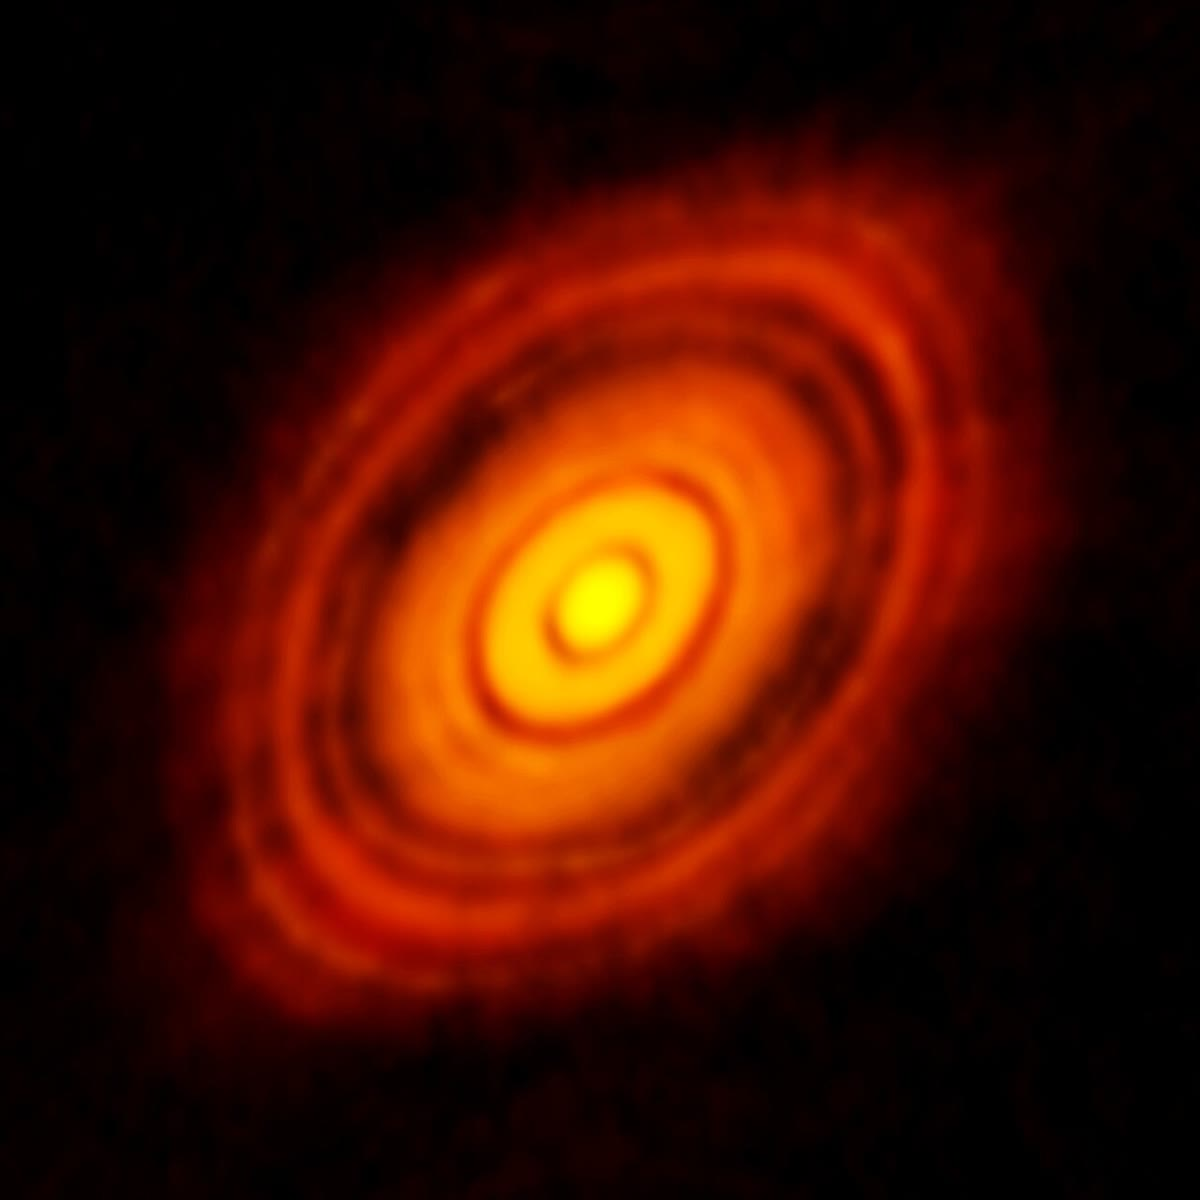
\includegraphics[width=\linewidth]{images/book4/b2-hl-tau-alma.jpg}
\end{minipage}\hfill
\begin{minipage}[c]{0.52\linewidth}
{\small Le disque de la jeune étoile HL Tauri, à \qty{140}{pc} dans le Taureau, photographié par
l'interféromètre ALMA à une longueur d'onde d'environ un millimètre, où la poussière froide brille. Le disque, d'environ \qty{120}{au} de rayon et vu incliné de \ang{47}, montre des anneaux
clairs et sombres larges de quelques unités astronomiques~; le système a au plus un ou deux millions d'années, et les anneaux sont interprétés comme les premiers signes de planètes qui dégagent leur trajectoire. ALMA (ESO/NAOJ/NRAO),
CC
BY
4.0.}
\end{minipage}
% ledger: alma:hltau
\end{omfigure}

Le disque est chauffé par l'étoile. Un grain situé à la distance $r$ absorbe la
lumière stellaire sur sa section et rayonne sur toute sa surface.

\begin{proposition}[Température d'un grain éclairé par une étoile]
\label{prop:b2:ism-star-formation:grain}
Un petit grain qui se comporte comme un corps noir, à la distance $r$ d'une étoile de
luminosité $L$ et éclairé par la lumière stellaire d'un seul côté, prend la température
\[
  T = \left(\frac{L}{16\pi\sigma r^2}\right)^{1/4},
\]
qui décroît comme $r^{-1/2}$.
\end{proposition}

\begin{proof}
Un grain sphérique de rayon $a$ intercepte la puissance $\pi a^2\,L/(4\pi r^2)$
et, à la température $T$, rayonne $4\pi a^2\sigma T^4$ sur sa surface. À l'équilibre les deux sont égales~: $T^4 = L/(16\pi\sigma r^2)$~; $a$ se
simplifie.
\end{proof}

À \qty{1}{au} d'une étoile semblable au Soleil, le grain est à \qty{278}{K}~; à
\qty{5.2}{au}, là où orbite Jupiter, à \qty{122}{K}. La glace d'eau se condense là où les grains sont plus froids que environ \qty{180}{K} (les températures de condensation
sont celles du \cref{ch:b2:planet-formation-meteorites}), c'est-à-dire au-delà d'environ \qty{2.4}{au}~: premier signe de la frontière, la ligne des glaces, qui sépare les planètes rocheuses des planètes glacées. Un disque réel est opaque, et son plan médian est à
l'abri de la lumière directe de l'étoile~; la proposition donne le bon ordre de grandeur et la bonne pente pour les couches de
surface
que
voit
l'étoile.
% ledger: lodders:tc-table

Les disques ne durent pas. L'excès infrarouge, la lueur de la poussière chaude au-delà de ce que
l'étoile émettrait seule, révèle si une étoile possède encore un disque. En comptant les étoiles qui présentent un tel excès dans des amas d'âges différents, on obtient la fraction des étoiles qui
conservent leur disque en fonction du temps (figure ci-dessous)~: la plupart des étoiles en ont un à la naissance, la moitié l'a perdu vers trois millions d'années, et presque aucune n'en garde un au-delà de six millions d'années. Les géantes gazeuses, qui doivent rassembler leur gaz à partir du disque,
doivent se former dans ces
quelques
millions
d'années.
% ledger: haisch:disc-fractions, haisch:disc-lifetime

\begin{omfigure}
\begin{tikzpicture}
\begin{axis}[omrecord, width=0.8\linewidth, height=5.6cm, xmin=0, xmax=8.5, ymin=0, ymax=1.05,
  xlabel={âge de l'amas (Ma)}, ylabel={fraction des étoiles avec un disque},
  tick label style={font=\scriptsize}, label style={font=\small}, clip=false]
\addplot[thick, black!55, densely dashed] table[x=age, y=frac] {figdata/out/bachelor-2-jeans-discfit.dat};
\addplot[only marks, mark=*, mark size=1.8pt, blue!70!black,
  error bars/.cd, y dir=both, y explicit]
  table[x=age, y=frac, y error=err, restrict x to domain=0:10] {figdata/out/bachelor-2-jeans-discs.dat};
\node[font=\scriptsize, anchor=north west] at (axis cs:0.05,0.74) {NGC 2024};
\node[font=\scriptsize, anchor=south west] at (axis cs:1.55,0.86) {Trapèze};
\node[font=\scriptsize, anchor=south west] at (axis cs:2.35,0.71) {IC 348};
\node[font=\scriptsize, anchor=south west] at (axis cs:3.3,0.56) {NGC 2264};
\node[font=\scriptsize, anchor=south west] at (axis cs:5.1,0.15) {NGC 2362};
\node[font=\scriptsize, anchor=north east] at (axis cs:8.4,0.98) {(NGC 1960, \qty{30}{Ma}~: $0.03$)};
\end{axis}
\end{tikzpicture}

\par\smallskip{\small Fraction des étoiles de jeunes amas qui montrent l'excès infrarouge
d'un disque, en fonction de l'âge de l'amas (avec son erreur), d'après Haisch, Lada et Lada (2001). La droite en pointillés est la droite des moindres carrés passant par les cinq
amas les plus jeunes~: elle atteint $0.5$ à \qty{3.0}{Ma} et zéro à
\qty{6.1}{Ma}
(\cref{exo:b2:ism-star-formation:12}).}
\end{omfigure}

\begin{inthelab}[Voir à travers la poussière avec les ondes radio]
\begin{minipage}[t]{0.55\linewidth}\vspace{0pt}
Le gaz froid et la poussière sont invisibles aux télescopes optiques, mais brillent aux
longueurs d'onde millimétriques, où l'atmosphère n'est transparente qu'au-dessus de sites élevés et secs. Une antenne parabolique de la taille d'une maison résout peu à ces longueurs
d'onde~; les astronomes en combinent donc plusieurs~: dans un interféromètre, chaque paire d'antennes, séparées par une base, mesure une composante de la figure de brillance du ciel, et un ordinateur assemble l'image à partir des centaines de paires que forment une
trentaine d'antennes. La résolution est celle d'un seul télescope aussi large que la plus longue base~: avec des antennes réparties sur \qty{15}{km}, le disque de HL Tauri a été imagé avec un détail de quelques unités astronomiques à \qty{140}{pc}. Les opérateurs déplacent les antennes sur des plateformes mobiles entre les configurations, et le corrélateur
combine
leurs
signaux
en
temps
réel.
\end{minipage}\hfill
\begin{minipage}[t]{0.42\linewidth}\vspace{0pt}
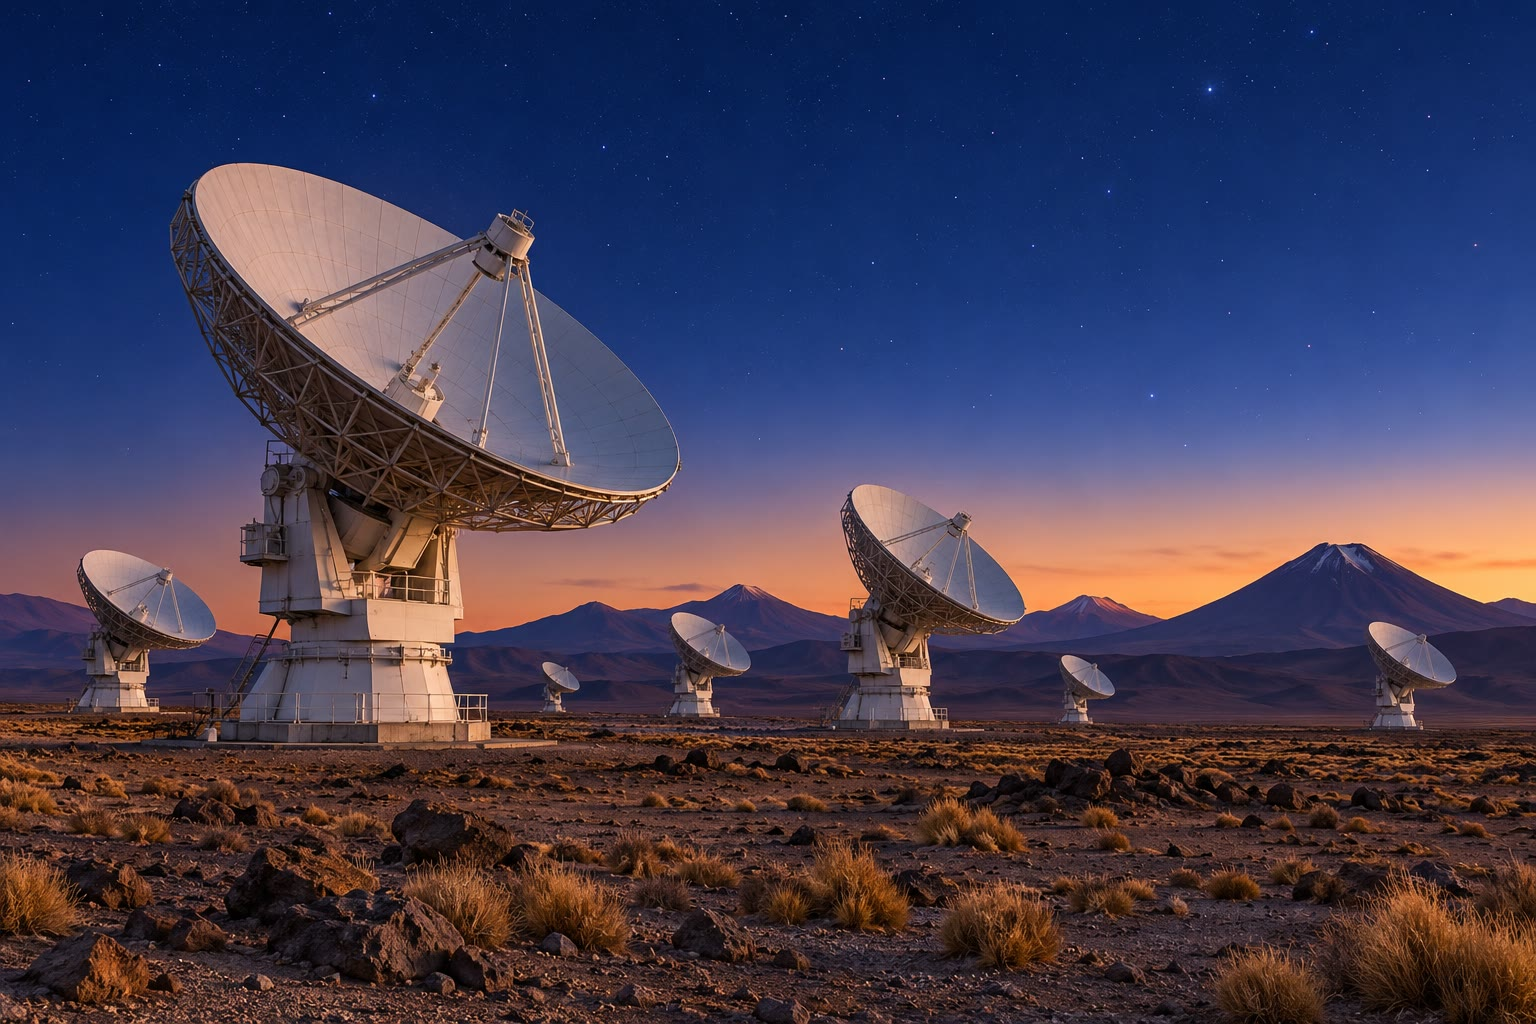
\includegraphics[width=\linewidth]{images/book4/ai/b2-radio-array.jpg}

{\scriptsize Un réseau d'antennes radio sur un haut plateau désertique au crépuscule
(Illustration générée par IA.)}
\end{minipage}
% ledger: alma:hltau, alma:baselines
\end{inthelab}

\section{Exercices}

\begin{exercise}[$\star$]\label{exo:b2:ism-star-formation:1}
La densité interstellaire moyenne près du Soleil vaut \qty{2.7e-24}{g.cm^{-3}}. La
masse d'un atome d'hydrogène étant \qty{1.67e-24}{g}, calculer le nombre d'atomes d'hydrogène par centimètre cube. Comparer ce nombre à celui des molécules par centimètre
cube dans l'air à \qty{101325}{Pa} et \qty{288}{K}
($n = P/k_{\mathrm B}T$).
% ledger: ferriere:mean-density, const:kB
\end{exercise}

\begin{exercise}[$\star$]\label{exo:b2:ism-star-formation:2}
À partir de la valeur $M_J = 5.46$ masses solaires à \qty{10}{K} et $10^4$ particules
par centimètre cube, et de la loi de variation de $M_J$ avec la densité, calculer la \omterm{def:b2:ism-star-formation:jeans}{masse de Jeans} à \qty{10}{K} et $10^2$ particules par centimètre cube. Combien de \omterm{def:b2:ism-star-formation:jeans}{masses
de Jeans} contient le nuage du Taureau, \num{24000} masses
solaires~?
% ledger: goldsmith:taurus-mass
\end{exercise}

\begin{exercise}[$\star$]\label{exo:b2:ism-star-formation:3}
Calculer la vitesse isotherme du son $c_s = (k_{\mathrm B}T/\mu m_u)^{1/2}$ dans un gaz
moléculaire ($\mu = 2.33$, $m_u = \qty{1.661e-27}{kg}$) à \qty{10}{K} et à \qty{100}{K}. Combien de temps une onde sonore met-elle pour traverser un cœur de rayon \qty{0.1}{pc}
à \qty{10}{K}, en millions
d'années~?
% ledger: kauffmann:mu, nist:u, iau:parsec
\end{exercise}

\begin{exercise}[$\star$]\label{exo:b2:ism-star-formation:4}
Calculer le \omterm{def:b2:ism-star-formation:free-fall}{temps de chute libre} d'un \omterm{def:b2:ism-star-formation:molecular-cloud}{cœur dense} de $10^5$ particules par centimètre
cube et celui d'un nuage sombre de $10^2$ ($\mu = 2.33$). Lequel s'effondre le plus vite, et de quel
facteur~?
\end{exercise}

\begin{exercise}[$\star\star$]\label{exo:b2:ism-star-formation:5}
Montrer que $M_J$ peut s'écrire $M_J = 5^{3/2}\,(3/4\pi)^{1/2}\,c_s^3\,G^{-3/2}\rho^{-1/2}$.
À température fixée, de quel facteur doit augmenter la densité d'un cœur pour que sa \omterm{def:b2:ism-star-formation:jeans}{masse
de Jeans} soit divisée par deux~? À densité fixée, de quel facteur la \omterm{def:b2:ism-star-formation:jeans}{masse de Jeans} change-t-elle si le cœur passe de \qty{10}{K} à
\qty{20}{K}~?
\end{exercise}

\begin{exercise}[$\star\star$]\label{exo:b2:ism-star-formation:6}
Une jeune étoile a la masse du Soleil, deux fois son rayon et deux fois sa luminosité
($M_\odot = \qty{1.989e30}{kg}$, $R_\odot = \qty{6.96e8}{m}$,
$L_\odot = \qty{3.83e26}{W}$). Calculer son \omterm{def:b2:ism-star-formation:kh-time}{temps de Kelvin--Helmholtz} en millions
d'années, et le comparer aux durées de vie des disques.
% ledger: sun:mass, sun:R, sun:L
\end{exercise}

\begin{exercise}[$\star\star$]\label{exo:b2:ism-star-formation:7}
Calculer le taux d'accrétion $c_s^3/G$ d'une \omterm{def:b2:ism-star-formation:protostar}{protoétoile} dans un cœur à \qty{10}{K}, en
masses solaires par an, et le temps qu'il faut pour rassembler une masse solaire. Mêmes questions pour un cœur à
\qty{20}{K}.
\end{exercise}

\begin{exercise}[$\star\star$]\label{exo:b2:ism-star-formation:8}
Avec la \cref{prop:b2:ism-star-formation:grain} et $L_\odot = \qty{3.83e26}{W}$, calculer
la distance au Soleil, en unités astronomiques, à laquelle un grain atteint \qty{1300}{K}, température voisine de celle à laquelle se condensent les silicates courants
(\cref{ch:b2:planet-formation-meteorites}), ainsi que la température d'un grain à la distance de
Jupiter,
\qty{5.2}{au}.
% ledger: sun:L, const:sigma, const:au
\end{exercise}

\begin{exercise}[$\star\star$]\label{exo:b2:ism-star-formation:9}
Le gaz du disque de HL Tauri tourne autour d'une étoile d'environ \num{1.3} masses
solaires. Calculer la vitesse képlérienne et la période orbitale à \qty{100}{au}. Si le système a un million d'années, combien de tours le gaz situé à \qty{100}{au} a-t-il
effectués depuis la naissance de
l'étoile~?
% ledger: alma:hltau
\end{exercise}

\begin{exercise}[$\star\star\star$]\label{exo:b2:ism-star-formation:10}
Calculer l'énergie gravitationnelle d'une sphère de rayon $R$ dans laquelle la densité
décroît comme $\rho(r) = \rho_0 R/r$, et la comparer à celle d'une sphère uniforme de même masse et de même rayon. La concentration de la masse vers le centre rend-elle le nuage
plus facile ou plus difficile à maintenir par son énergie
thermique~?
\end{exercise}

\begin{exercise}[$\star\star\star$]\label{exo:b2:ism-star-formation:11}
Un cœur de rayon \qty{0.1}{pc} tourne en bloc, comme un solide, à la vitesse angulaire
$\Omega = \qty{1e-14}{rad.s^{-1}}$. Calculer sa période de rotation, le moment cinétique massique $j = \Omega R^2$ du gaz situé à son équateur et le rayon centrifuge de ce
gaz autour d'une étoile d'une masse solaire, en unités astronomiques. Pourquoi le gaz venant de l'intérieur du cœur tombe-t-il plus près
de
l'étoile~?
\end{exercise}

\begin{exercise}[$\star\star\star$]\label{exo:b2:ism-star-formation:12}
Les fractions de disques des cinq amas les plus jeunes de la figure de la dernière
section valent $0.85$, $0.80$, $0.65$, $0.52$ et $0.12$ à 0.3, 1.5, 2.3, 3.2 et \qty{5.0}{Ma}. Ajuster à la main une droite des moindres carrés $f = a - bt$ (calculer
les moyennes, puis $\sum(t - \bar t)(f - \bar f)$ et $\sum(t - \bar t)^2$). À quel âge atteint-elle la moitié, puis zéro~? Pourquoi une droite est-elle un mauvais modèle au-delà
de
cet
âge~?
% ledger: haisch:disc-fractions
\end{exercise}

\section{Problème~: un cœur du nuage d'Aldra}

\begin{problem}[{Problème du week-end --- la masse et la stabilité d'un cœur dense lues sur une carte
de poussière, la naissance de sa protoétoile et la taille de son disque}]
\label{pb:b2:ism-star-formation:1}
% values: calc/ch01.py
% ledger: kauffmann:mu, nist:u, iau:parsec, const:G, const:kB, sun:mass, sun:R, sun:L, const:au, const:sigma, bt07:cores, alma:hltau
Le nuage d'Aldra est un nuage sombre inventé. Une carte millimétrique de sa
poussière montre un cœur rond de rayon \qty{0.08}{pc}, de densité de colonne moyenne $N(\ce{H2}) = \num{1.5e22}$ molécules d'hydrogène par centimètre carré.
Une raie de l'ammoniac donne la température du gaz, \qty{10}{K}, et un gradient de vitesse de \qty{0.4}{km.s^{-1}} par parsec à travers le cœur, lu comme une rotation solide. Utiliser $G = \qty{6.674e-11}{m^3.kg^{-1}.s^{-2}}$,
$k_{\mathrm B} = \qty{1.381e-23}{J.K^{-1}}$, $m_u = \qty{1.661e-27}{kg}$, \qty{1}{pc} $= \qty{3.086e16}{m}$, \qty{1}{au} $= \qty{1.496e11}{m}$, une année de \qty{3.156e7}{s}, $M_\odot = \qty{1.989e30}{kg}$, $R_\odot = \qty{6.96e8}{m}$, $L_\odot = \qty{3.83e26}{W}$, $\sigma = \qty{5.67e-8}{W.m^{-2}.K^{-4}}$~;
la masse par molécule d'hydrogène, hélium compris, vaut $2.8\,m_u$,
et
la
masse
moyenne
par
particule
$2.33\,m_u$.

\medskip
\noindent\textbf{Partie I --- Masse et densité.}
\begin{enumerate}
  \item Convertir le rayon du cœur en mètres.
  \item Calculer la masse par mètre carré de la colonne, $2.8\,m_u N$.
  \item En déduire la masse du cœur, en kilogrammes et en masses solaires.
  \item Calculer son volume et sa densité moyenne.
  \item Calculer le nombre de particules par centimètre cube.
  \item Ce cœur est-il un \omterm{def:b2:ism-star-formation:molecular-cloud}{cœur dense} au sens du tableau de la deuxième section~?
\end{enumerate}

\noindent\textbf{Partie II --- Stabilité.}
\begin{enumerate}[resume]
  \item Calculer la \omterm{def:b2:ism-star-formation:jeans}{masse de Jeans} du gaz du cœur, en masses solaires.
  \item Combien de \omterm{def:b2:ism-star-formation:jeans}{masses de Jeans} le cœur contient-il~? Est-il stable~?
  \item Calculer la \omterm{def:b2:ism-star-formation:jeans}{longueur de Jeans} et la comparer au rayon du cœur.
  \item Quelle serait la \omterm{def:b2:ism-star-formation:jeans}{masse de Jeans} si le gaz était à \qty{20}{K}~? Le cœur
        s'effondrerait-il encore~?
  \item Calculer le \omterm{def:b2:ism-star-formation:free-fall}{temps de chute libre} du cœur, en milliers d'années.
  \item Le comparer au temps qu'une onde sonore met à traverser le cœur. Quel
        processus est le plus rapide, et qu'est-ce que cela signifie~?
\end{enumerate}

\noindent\textbf{Partie III --- La protoétoile.}
\begin{enumerate}[resume]
  \item Calculer la vitesse du son dans le cœur.
  \item Calculer le taux d'accrétion $c_s^3/G$, en masses solaires par an.
  \item Calculer le temps nécessaire pour rassembler une masse solaire à ce taux.
  \item Si un tiers du cœur finit en étoiles, combien d'étoiles d'une masse solaire
        peut-il en former~?
  \item Une fois l'enveloppe dissipée, l'étoile a une masse solaire, trois rayons
        solaires et quatre luminosités solaires. Calculer son \omterm{def:b2:ism-star-formation:kh-time}{temps de Kelvin--Helmholtz}.
  \item Est-il plus long ou plus court que le temps d'accrétion~? De quel type d'étoile
        s'agit-il alors~?
\end{enumerate}

\noindent\textbf{Partie IV --- Le disque.}
\begin{enumerate}[resume]
  \item Convertir le gradient de vitesse en une vitesse angulaire $\Omega$, en
        \unit{rad.s^{-1}}.
  \item Calculer le moment cinétique massique $j = \Omega R^2$ du gaz situé à l'équateur
        du cœur.
  \item Calculer son rayon centrifuge autour d'une étoile d'une masse solaire, en
        unités astronomiques.
  \item Calculer la température d'un grain à \qty{1}{au} et à \qty{30}{au}
        d'une étoile de luminosité solaire.
  \item Où se situe la ligne des glaces de ce disque, si la glace d'eau subsiste sous
        \qty{180}{K}~?
  \item Donner le temps nécessaire pour assembler l'étoile de la question 15, le nombre
        clé de ce problème, en milliers d'années, et le comparer au \omterm{def:b2:ism-star-formation:free-fall}{temps de chute libre}
        de la question 11.
\end{enumerate}
\end{problem}
